% First Chapter


\ifpdf
    \graphicspath{{Chapter1/Figs/Raster/}{Chapter1/Figs/PDF/}{Chapter1/Figs/}}
\else
    \graphicspath{{Chapter1/Figs/Vector/}{Chapter1/Figs/}}
\fi

\chapter{Introduction to Data Quality}

A Web search of terms "data quality" through the search engine Google, returns about three millions of pages
and indicator that data quality issues are real and increasingly important (the term data quality will be shortened to the acronym DQ)

\ifpdf
    \graphicspath{{Chapter1/Figs/Raster/}{Chapter1/Figs/PDF/}{Chapter1/Figs/}}
\else
    \graphicspath{{Chapter1/Figs/Vector/}{Chapter1/Figs/}}
\fi

\section{Introduction to the Concept of Data Quality}

From a research perspective, data quality has been addressed in different
areas, including statistics, management, and computer science. Statisticians were the first to investigate some of the problems related to data quality, by
proposing a mathematical theory for considering duplicates in statistical data sets, in the late 1960's. They were followed by researchers in management, who
at the beginning of the 1980's focused on how to control data manufacturing systems in order to detect and eliminate data quality problems. Only at the
beginning of the 1990's computer scientists begin considering the problem of defining, measuring, and improving the quality of electronic data stored in
databases, data warehouses, and legacy systems.~\citep{CBMS}

Dr. Genichi Taguchi~\citep{Jugulum14}, who was a world-renowned quality engineering expert from Japan, emphasized and established the relationship between
poor quality and overall loss. Dr. Taguchi (1987) used a quality loss function (QLF) to measure the loss associated with quality characteristics
or parameters. The QLF describes the losses that a system suffers from an adjustable characteristic. According to the QLF, the loss increases as
the characteristic y (such as thickness or strength) gets further from the target value (m). In other words, there is a loss associated if the quality
characteristic diverges from the target. Taguchi regards this loss as a loss to society, and somebody must pay for this loss. The results of such losses
include system breakdowns, company failures, company bankruptcies, and so forth.

Figure 1.1 shows how the loss arising from varying (on either side)
from the target by $\Delta_0$ increases and is given by $L(y)$ when $y$ is equal to $m$,

\begin{figure}[htbp!] 
\centering    
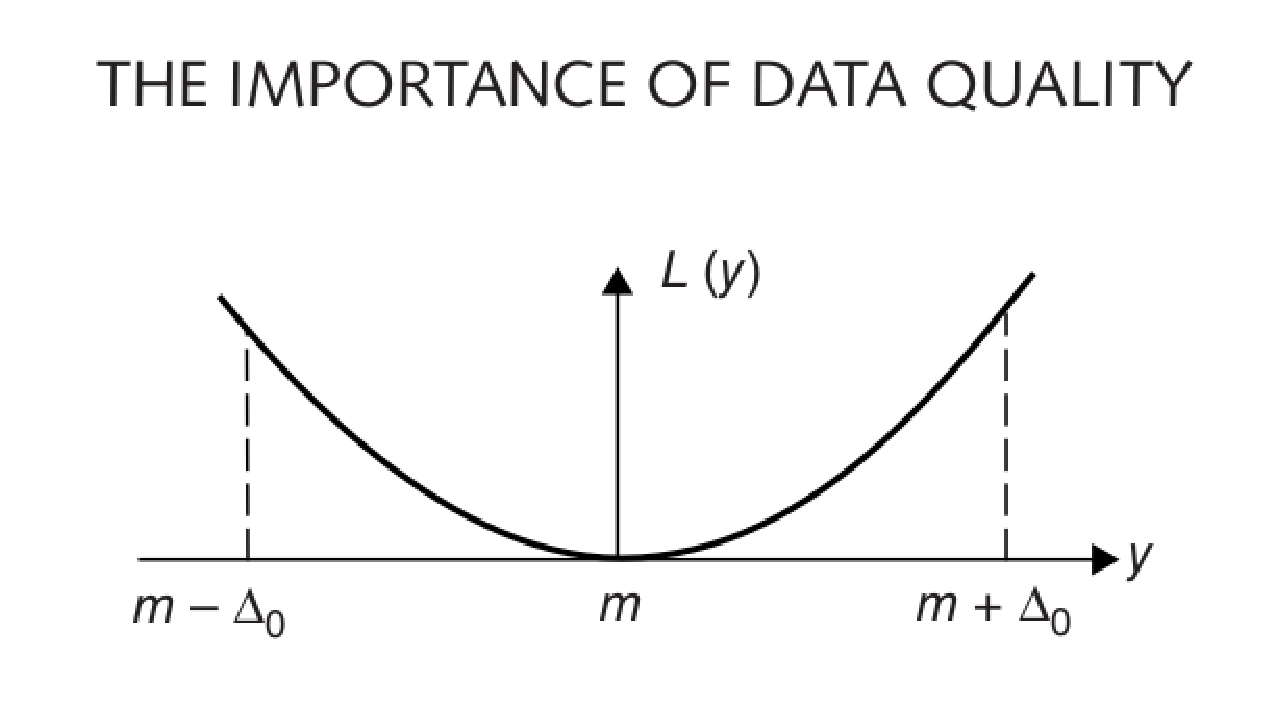
\includegraphics[width=0.6\textwidth]{quality-loss-function}
\caption{Quality Loss Function (QLF)}
\end{figure}

the loss is zero, or at the minimum. The equation for the loss function can
be expressed as follows:

\begin{equation*}
    L(y) = k(y-m)^2
\end{equation*}

where $k$ is a factor that is expressed in dollars, based on direct costs, indirect costs, 
warranty costs, reputational costs, loss due to lost customers,
and costs associated with rework and rejection. There are prescribed ways
to determine the value of $k$.
The loss function is usually not symmetrical-sometimes it is steep on
one side or on both sides. Deming ~\citep{Deming} says that the loss function need
not be exact and that it is difficult to obtain the exact function. As most
cost calculations are based on estimations or predictions, an approximate
function is sufficient-that is, close approximation is good enough.

The concept of the loss function aptly applies in the DQ context, especially when we are measuring data quality associated with various data
elements such as customer IDs, social security numbers, and account balances. Usually, the data elements are prioritized based on certain criteria,
and the quality levels for data elements are measured in terms of percent-
ages (of accuracy, completeness, etc.). The prioritized data elements are
referred to as critical data elements (CDEs).

\section{Why Data Quality is Relevant}

The consequences of poor quality of data are often experienced in everyday life, but often, without making the necessary connections to their causes.

For example, the late or mistaken delivery of a letter is often blamed on a postal service, although  a closer look often reveals data-related causes, typically an error in the address, orginating in the address database.

Data quality has serious consequences of far-reaching significance, for the efficiency and effectiveness of organizations and business.


\section{Why Data Quality is Matters}

Poor data quality is enemy number one to the widespread, profitable use of machine learning. While the caustic observation, “garbage-in, garbage-out” has plagued analytics and decision-making for generations, it carries a special warning for machine learning. The quality demands of machine learning are steep, 
and bad data can rear its ugly head twice - first in the historical data used to train the predictive model and second in the new data used by that model to make future decisions. ~\cite{RedmanHBR2018}

Data quality is no less troublesome in implementation. Consider an organization seeking productivity gains with its machine learning program. While the data science team that developed the predictive model may have done a solid job cleaning the training data, it can still be compromised by bad data going forward. Again, it takes people — lots of them — to find and correct the errors. This in turns subverts the hoped-for productivity gains. Further, as machine learning technologies penetrate organizations, 
the output of one predictive model will feed the next, and the next, and so on, even crossing company boundaries. The risk is that a minor error at one step will cascade, causing more errors and growing ever larger across an entire process.

\begin{figure}[H]
    \centering
    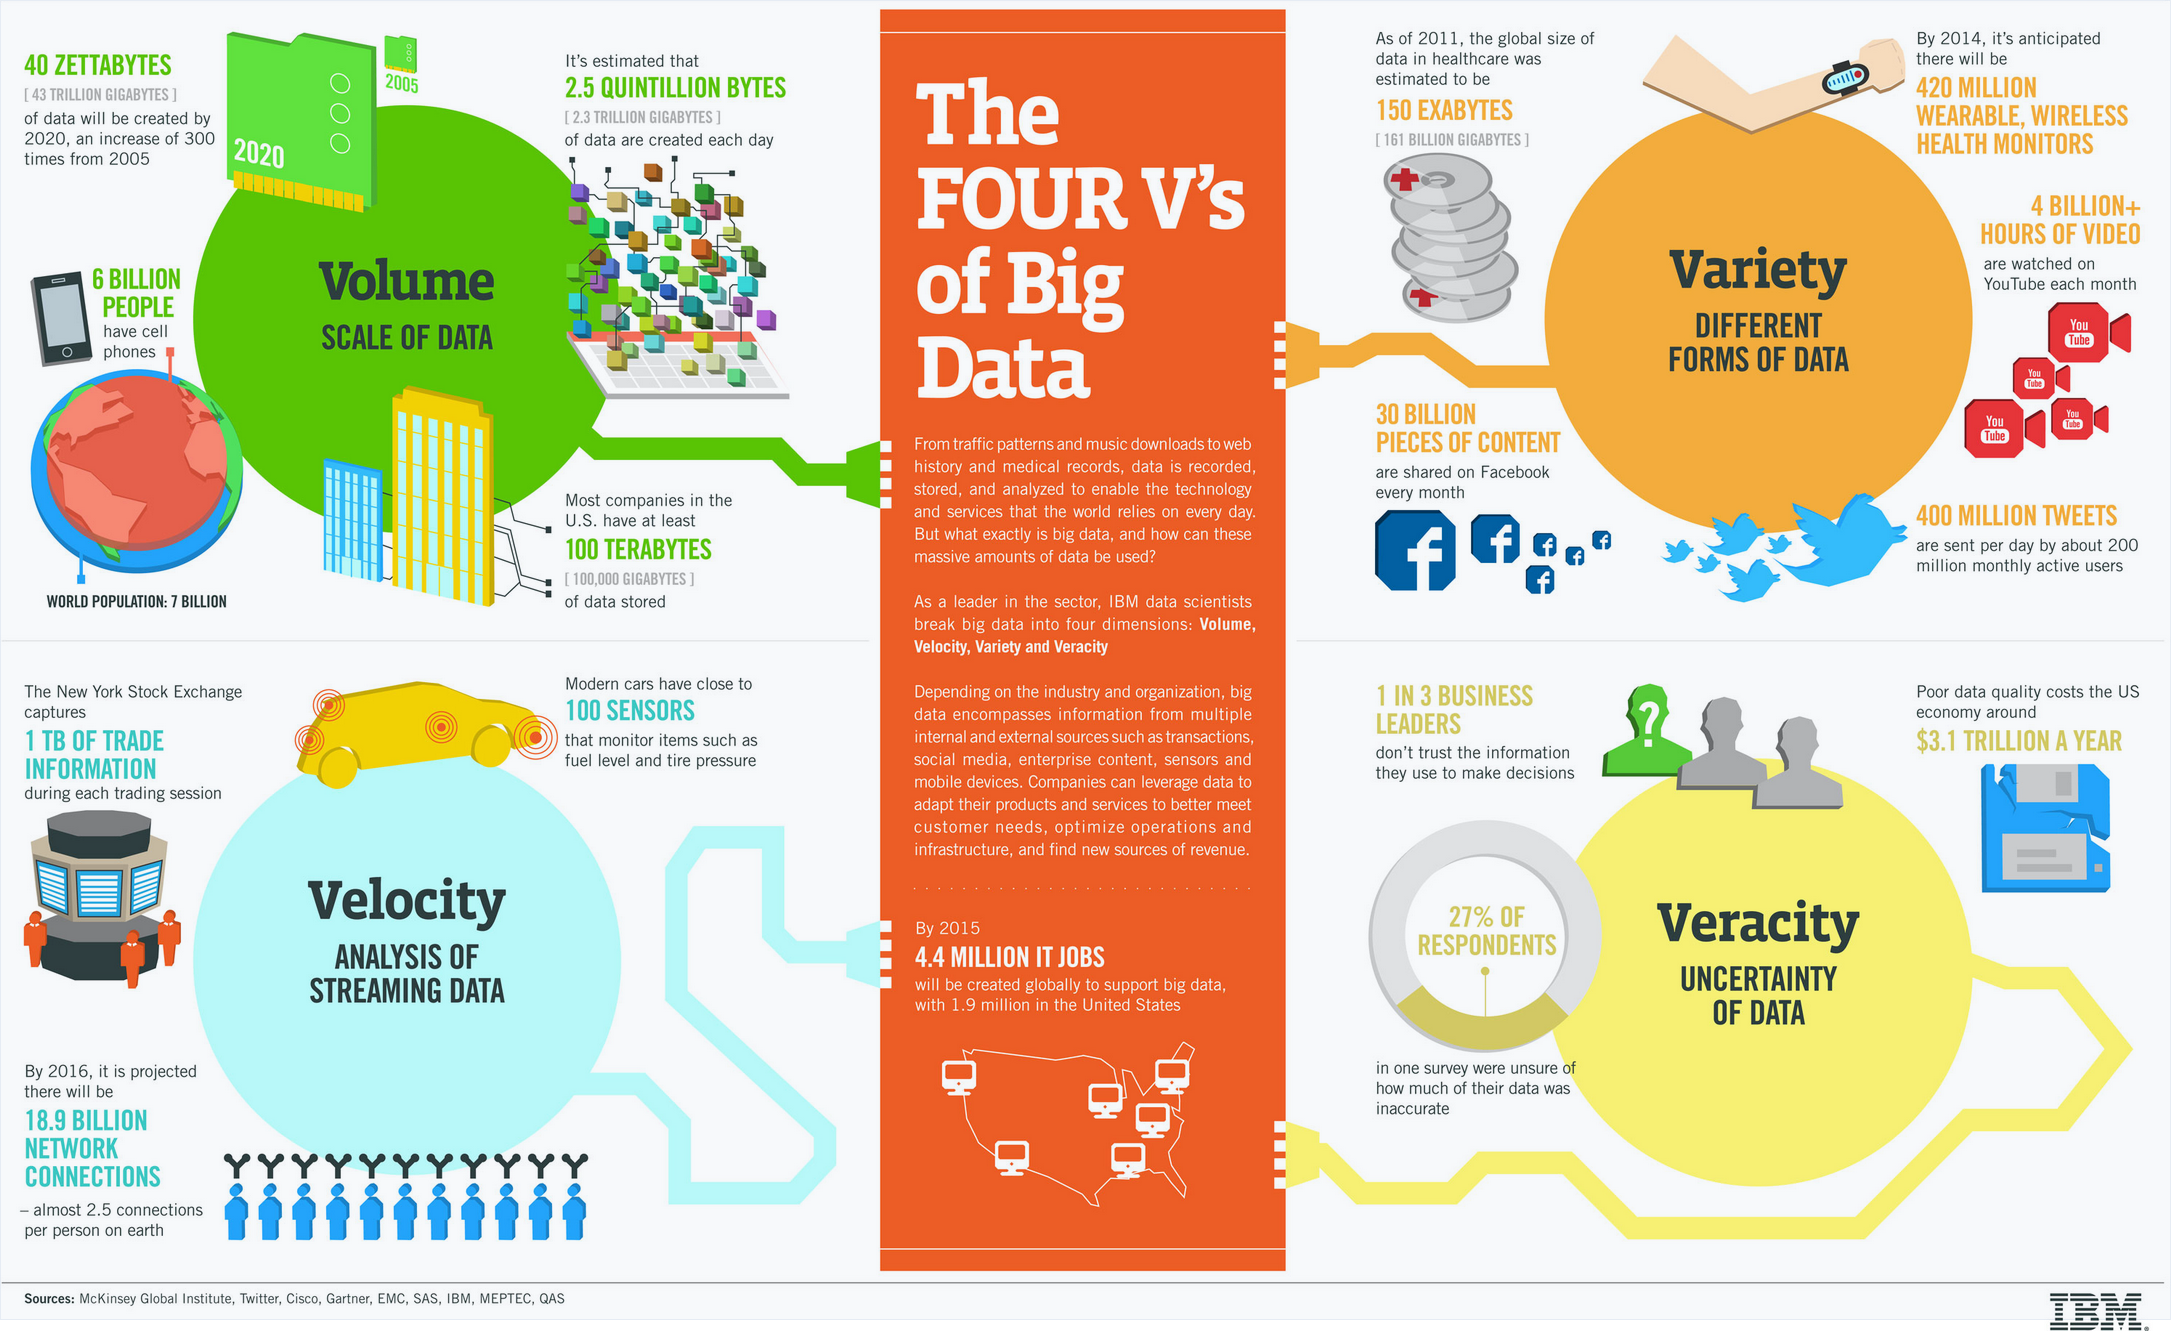
\includegraphics[angle=-90,scale=.3]{4-Vs-of-big-data}
    \caption{IBM data scientists break big data into four dimensions: volume, variety, velocity and veracity. This infographic explains and gives examples of each. ~\cite{ibmInfoGraphic}}
\end{figure}



\section{Data Quality and Types of Information Systems}

Data are collected, stored, elaborated, retrieved, and exchanged in information systems used in organizations to provide services to business processes.
Different criteria can be adopted for classifying the different types of information systems, and their corresponding architectures; they are usually related to
the overall organizational model adopted by the organization or the set of the
organizations that make use of the information system.

The three classifications are represented together in the classification space of Figure 1.2.
Among all possible combinations, five main types of information systems are highlighted in the figure:
Monolithic, Distributed, Data Warehouses,Cooperative, and Peer-to-Peer.

\begin{itemize}
    \item{In a \textit{monolithic information system} presentation, application logic, and data management are merged into a single computational node.
    Many monolithic information systems are still in use. While being extremely rigid, they provide advantages to organizations, such as reduced costs due to homogenetiy of solutions and centralization of management.
    In monolithic systems data flows have a common format, and data quality control is facilitated by the homogenetiy and centralization of procedures and management rules.}
    \item {A \textit{data warehouse} (DW) is a centralized set of data collected from different sources, designed to support management decision making. The most critical problem in DW design concerns the cleaning and integration of 
    the different data sources that are loaded into the DW, in that much of the implementation budget is spent on data cleaning activities.}
    \item{A \textit{distributed information system} relaxes the rigid centralization of monolithic systems, in that it allows the distribution of resources and applications across
    network of geographically distributed systems.
    The network can be organized in terms of several tiers, each made of one or more computational nodes. Presentation, application logic, and data management are distributed across tiers. Usually, the different tiers and nodes have a limited degree of autonomy, 
    data design is usually performed centrally, but to a certain extent some degree of heterogenetiy can occur, due to the impossibility of establishing unified procedures.
    Problems of data management are more complex than in monolithic systems, due to the reduced level of centralization.
    }  
\end{itemize}

\begin{figure}[H]
% \vspace*{.0in}
\centering
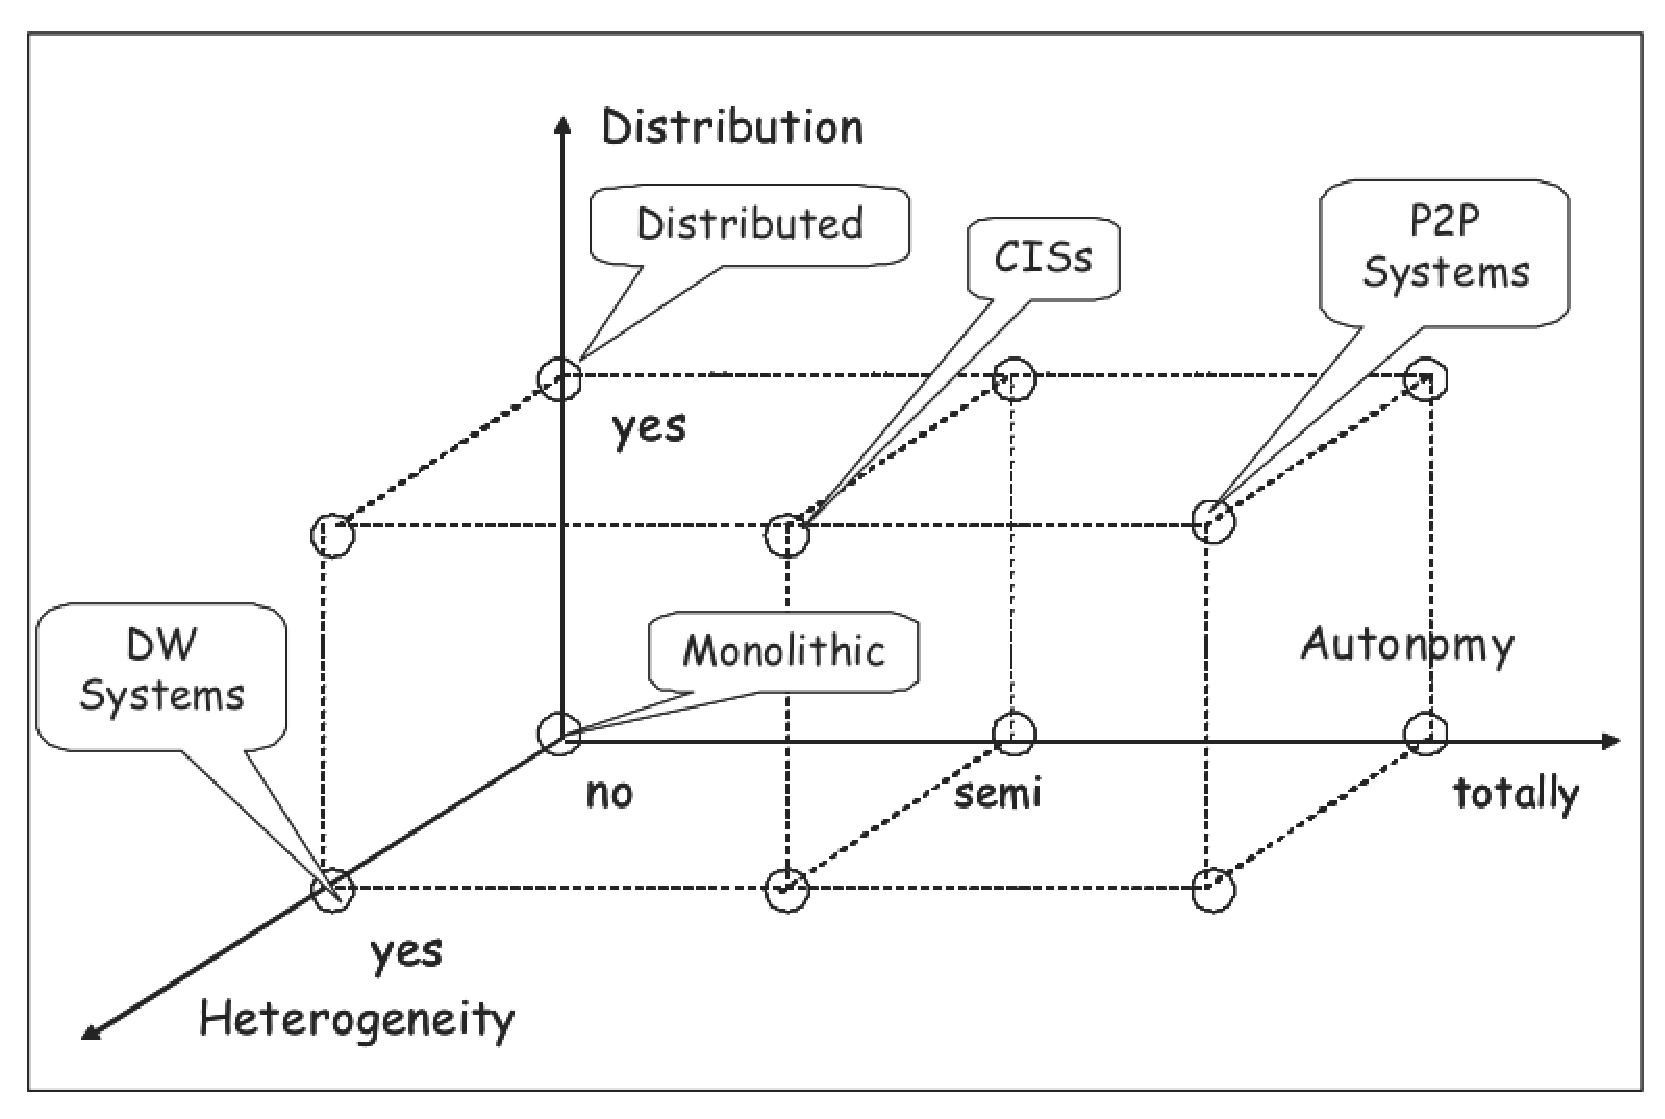
\includegraphics[scale=.50]{types-of-information-systems}
\caption{Types of information systems}    
\end{figure}

\begin{itemize}
    \item{A \textit{coorparative information system} (CIS) can be defined as a large-scale information system that interconnects various systems of different and autonomous organizations, 
    while sharing common objectives.}
    \item{In a \textit{peer to peer information system} (usually abbreviated P2P), the traditional distinction between clients and servers typical of distributed systems is disappearing.
    A P2P system can be characterized by a number of properties: peers are highly autonomous and higly heterogeneous, they have no obligation for the quality of their services
    and data, no central coordination and no central database exist, no peer has a global view of the system, global behavior emerges from local intreactions.    
    }
\end{itemize}


\section{Main Research Issues and Application Domains in Data Quality}
Due to the relevance of data quality, its nature, and the variety of data types and information systems, achieving data quality is a complex, multidisciplinary 
area of investigation. I involves several research topics and real-life application areas

\begin{figure}[H]
%\vspace*{.0in}
\centering
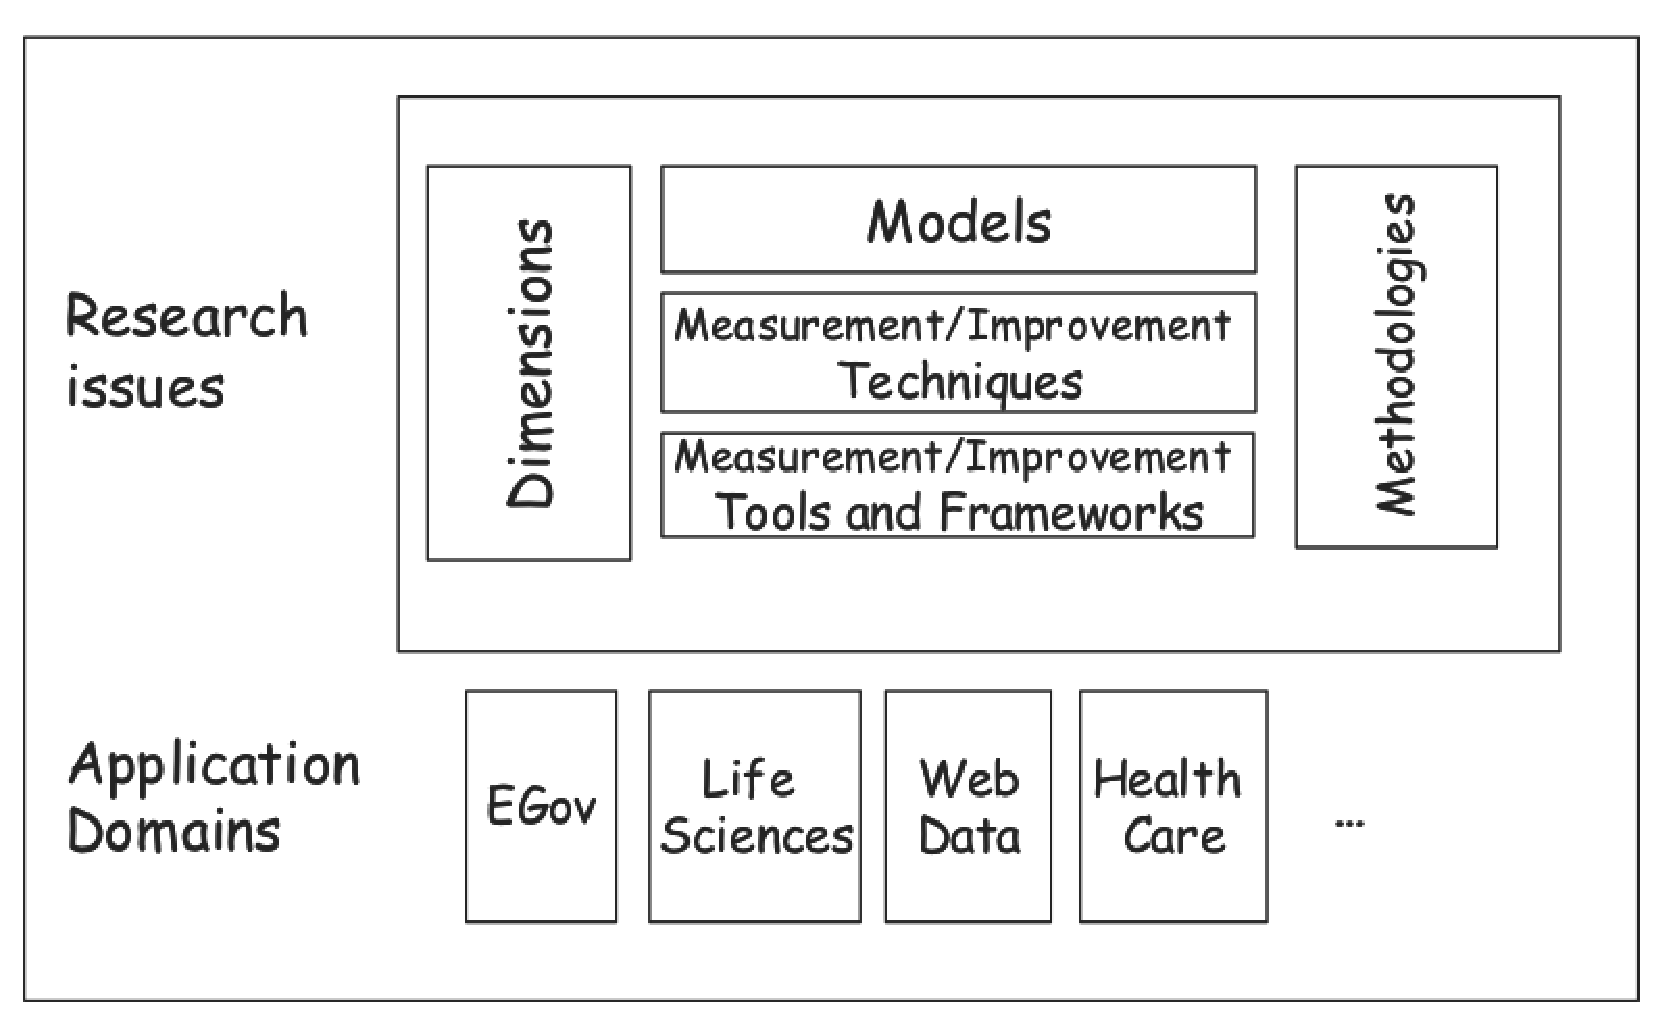
\includegraphics[scale=.50]{main-issues-in-dq}
\caption{Main issues in data quality}    
\end{figure}